\section*{QUESTION \quesNo.}

\subsection*{Explanation/Theory}

As obvious, the term consists of two words, 
'Amplitude' which means the maximum value of a signal and 
'Modulation' which means the process of varying the signal. 
So, Amplitude Modulation is the process of varying the amplitude of a signal. 
For example, in the case signal $y(t) = a_m(t)x(t)$ where $x(t) = A \sin(2\pi f t)$,
the amplitude of the input signal is $A$ and the frequency of the signal is $f$. \\
$a_m(t)$ is the modulating signal which is multiplied with the input signal to get the modulated signal.
Thus, this Amplitute of the output signal is varied by the modulating signal.


\subsection*{MATLAB Code}

\lstinputlisting[
    style=Matlab-Pyglike
]{matlab/22016_1.m}


\subsection*{Output}
\begin{figure}[H]
    \centering
    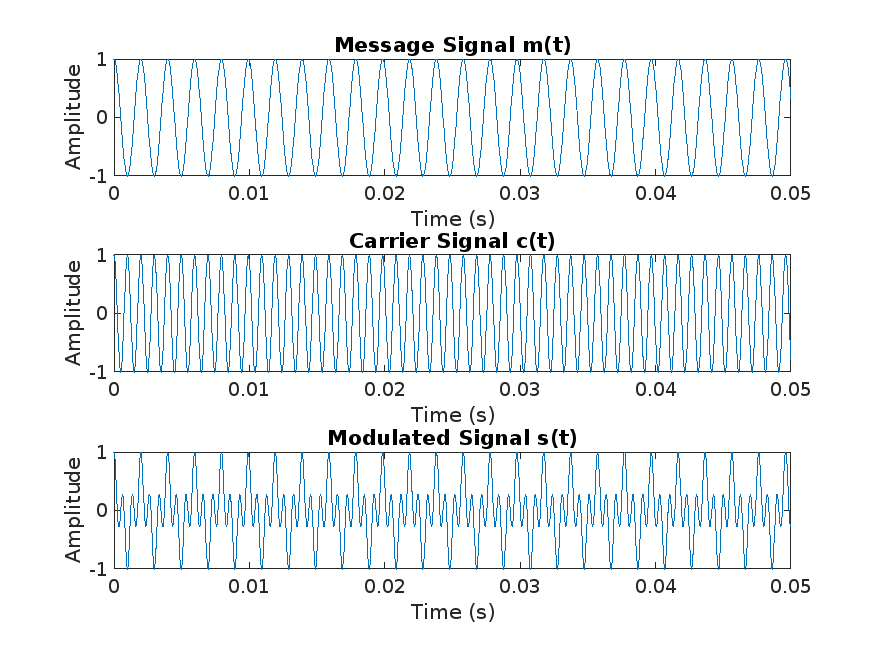
\includegraphics[width = .49\textwidth]{./imgs/1_individual_signals.png}\hfill
    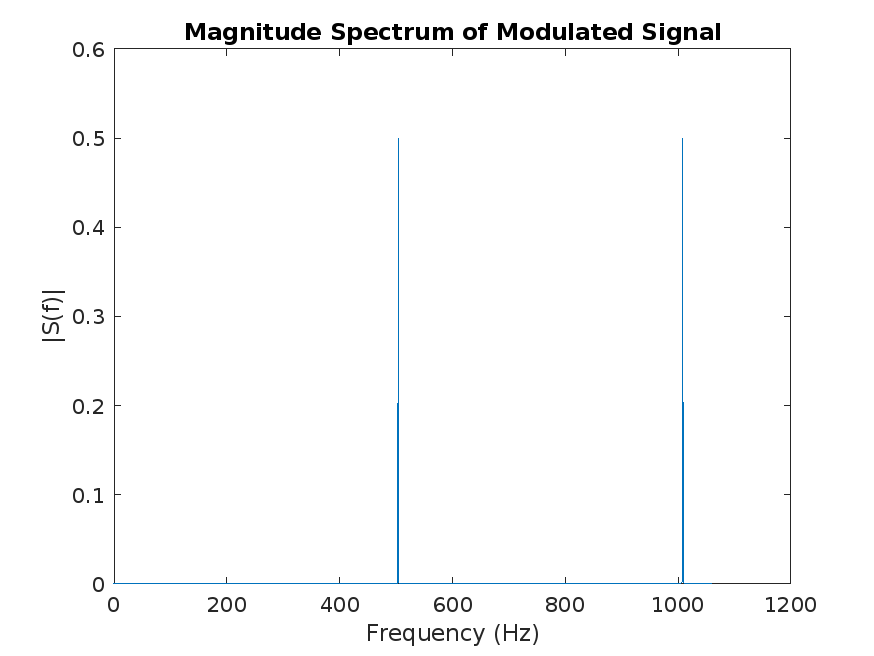
\includegraphics[width = .49\textwidth]{./imgs/1_magnitude_spectrum.png}
    \caption{Individual Signals and Magnitude Spectrum}
\end{figure}


\subsection*{Inference}
\begin{enumerate}
    \item The amplitude of the output signal is varied by the modulating signal.
    \item The phase of the output signal is same as the phase of the input signal.
    \item The amplitude of the output signal is same as the max product of amplitude of the input signal and amplitude of the modulating signal.
\end{enumerate}